\question (南京理工大学,2000年)归并排序中,归并趟数的数量级是( )
\par\fourch{}{\textcolor{red}{}}{}{}
\begin{solution}第一趟是2个一组; 第二趟是4个一组; \ldots{}\ldots{}
第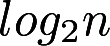
\includegraphics[width=0.40625in,height=0.14583in]{texmath/11a3d45Cdpi7B3507Dlog_2n}趟是n个一组;
\end{solution}
\question (北京航空航天大学,2007年)对具有n个元素的序列采用二路归并排序算法排序,算法的空间复杂度是(
)
\par\fourch{\textcolor{red}{}}{}{}{}
\begin{solution}常见排序算法的空间复杂度如下:
快速排序: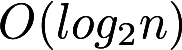
\includegraphics[width=0.65625in,height=0.18750in]{texmath/39368f5Cdpi7B3507DO28log_2n29}归并排序:O(n)
基数排序:O(rd) 其他:O(1)
\end{solution}
\question (北京师范大学,2004年)用某种排序方法对线性表\{24,88,21,48,15,27,69,35,20\}进行排序时,元素序列的变化情况如下:
(1)24,88,21,48,15,27,69,35,20 (2)20,15,21,24,48,27,69,35,88
(3)15,20,21,24,35,27,48,69,88 (4)15,20,21,24,27,35,48,69,88
则所采用的排序方法是( )
\par\twoch{\textcolor{red}{快速排序}}{选择排序}{希尔排序}{归并排序}
\begin{solution}如果是选择排序,则在4轮排序过程中无法得到最后的排序结构。如果是希尔排序不可能在第一步将20换到第一位。同理也不是归并排序。这4次过程中是子序列同时进行的快速排序
\end{solution}
\question (山东大学,2004年)将两个各有n个元素的有序表归并成一个有序表,其最少的比较次数是(
)
\par\twoch{\textcolor{red}{n}}{2n-1}{2n}{n-1}
\begin{solution}最小的情况就是一个有序表的最小元素比另外一个有序表的最大元素还要大,这样需要比较n次,则可以将两个序列归并。
\end{solution}
\question (华南理工大学,2006年)对各种内部排序方法来说,( )
\par\twoch{快速排序时间性能最佳}{\textcolor{red}{基数排序和归并排序是稳定的排序方法}}{快速排序是一种选择排序}{堆排序使用的辅助空间比较大}
\begin{solution}A快速排序在一定情况下时间复杂度会退化为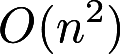
\includegraphics[width=0.43750in,height=0.19792in]{texmath/ead2f65Cdpi7B3507DO28n5E229},B正确,C选择排序即最简单的选出一个最大(最小)数据的排序方式,并非快速排序。D堆排序需要的额外存储空间为O(1),是最小的情况
\end{solution}
\question (中国科学院,2007年)若要求在O(nlogn)的时间内完成对数组的排序,且要求是稳定的,则可选择的排序方法是(
)
\par\twoch{快速排序}{堆排序}{\textcolor{red}{归并排序}}{直接插入排序}
\begin{solution}快速排序和堆排序不稳定,直接插入排序的时间复杂度是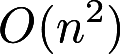
\includegraphics[width=0.43750in,height=0.19792in]{texmath/ead2f65Cdpi7B3507DO28n5E229}
\end{solution}
